\subsection{Cen�rio Detec��o de Cortes \label{use_case_cortes}}

\begin{figure}[h|top]
 \centering
 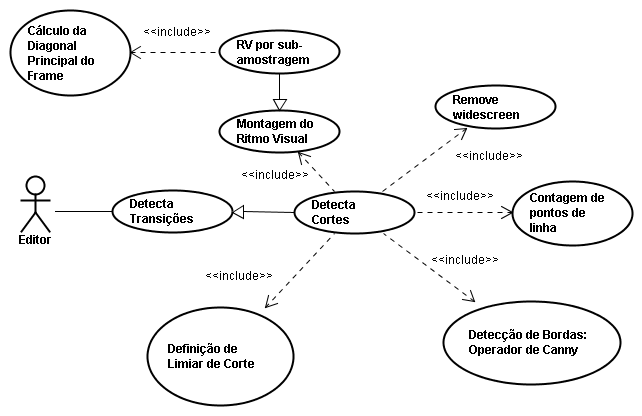
\includegraphics[width=1.0\linewidth]{imagens/use_case_cortes.png}
 \caption{Caso de Uso para cen�rio de detec��o de cortes.}
 \label{img_use_case_cortes}
\end{figure}

A Figura \ref{img_use_case_cortes}, representa o cen�rio espec�fico
de detec��o de cortes.

\subsubsection{Caso de uso: Detecta Cortes \label{use_case_detecta_cortes}}

\textbf{Cen�rio Principal:} Feito o carregamento do v�deo, o
processo de detec��o de transi��es se iniciar� pela detec��o de
cortes.

\subsubsection{Caso de uso: Montagem do Ritmo Visual por sub-amostragem \label{use_case_rv_amostra}}

\textbf{Cen�rio Principal:} Para a realiza��o da detec��o de cortes,
o sistema monta o Ritmo Visual do v�deo atrav�s da extra��o de
sub-amostragens de todos os frames do v�deo.

\subsubsection{Caso de uso: C�lculo da diagonal principal do frame \label{use_case_diagonal_principal}}

\textbf{Cen�rio Principal:} � realizado o c�lculo da diagonal
principal de cada frame do v�deo devido � necessidade de montar o
Ritmo Visual do v�deo.

\subsubsection{Caso de uso: Filtragem: Diminui��o de Ru�dos \label{use_case_filtragem}}

\textbf{Cen�rio Principal:} Montado o Ritmo Visual do v�deo, o
sistema realiza a filtragem da imagem do Ritmo Visual, com o
objetivo de eliminar poss�veis ru�dos existentes na imagem.

\subsubsection{Caso de uso: Detec��o de Bordas: Operador Sobel \label{use_case_sobel}}

\textbf{Cen�rio Principal:}
